\section{Schema del Database}

\subsection{Panoramica del Sistema}
Il database CoWorkSpace è progettato per gestire un sistema completo di prenotazione di spazi di coworking. La struttura supporta:
\begin{itemize}
    \item Gestione utenti con ruoli differenziati (utente, manager, admin)
    \item Gestione di più sedi (locations) con relativi manager
    \item Tipologie di spazi flessibili e personalizzabili
    \item Sistema di prenotazioni con gestione pagamenti
    \item Sistema di notifiche multi-canale
    \item Gestione disponibilità spazi per giorno
\end{itemize}

\subsection{Tipi ENUM Personalizzati}
Il sistema utilizza diversi tipi ENUM per garantire coerenza dei dati:

\begin{lstlisting}[caption=Definizione Tipi ENUM]
-- Ruoli utente
CREATE TYPE user_role_enum AS ENUM ('user', 'manager', 'admin');

-- Stati prenotazione
CREATE TYPE booking_status_enum AS ENUM ('confirmed', 'pending', 'cancelled', 'completed');

-- Stati pagamento
CREATE TYPE payment_status_enum AS ENUM ('pending', 'completed', 'failed', 'refunded');

-- Metodi di pagamento
CREATE TYPE payment_method_enum AS ENUM ('credit_card');
\end{lstlisting}

\newpage

\subsection{Entità Principali}

\subsubsection{Tabella Users}
Gestisce tutti gli utenti del sistema con autenticazione e autorizzazione.

\begin{lstlisting}[caption=Struttura Tabella Users]
CREATE TABLE users (
  user_id SERIAL PRIMARY KEY,
  name VARCHAR(100) NOT NULL,
  surname VARCHAR(100) NOT NULL,
  email VARCHAR(255) UNIQUE NOT NULL CHECK (email ~* '^[A-Za-z0-9._%+-]+@[A-Za-z0-9.-]+\.[A-Za-z]{2,}$'),
  password_hash VARCHAR(255) NOT NULL,
  role user_role_enum NOT NULL DEFAULT 'user',
  is_password_reset_required BOOLEAN DEFAULT FALSE,
  temp_password_hash VARCHAR(255),
  temp_password_expires_at TIMESTAMP,
  fcm_token VARCHAR(255),
  manager_request_pending BOOLEAN DEFAULT FALSE,
  manager_request_date TIMESTAMP,
  created_at TIMESTAMP DEFAULT CURRENT_TIMESTAMP
);
\end{lstlisting}

\textbf{Caratteristiche principali:}
\begin{itemize}
    \item Validazione email tramite regex
    \item Gestione reset password temporanee
    \item Support per notifiche push (FCM token)
    \item Sistema di richiesta promozione a manager
\end{itemize}

\subsubsection{Tabella Locations}
Rappresenta le sedi fisiche dove si trovano gli spazi di coworking.

\begin{lstlisting}[caption=Struttura Tabella Locations]
CREATE TABLE locations (
  location_id SERIAL PRIMARY KEY,
  location_name VARCHAR(255) NOT NULL,
  address VARCHAR(255) NOT NULL,
  city VARCHAR(100) NOT NULL,
  description TEXT,
  manager_id INT,
  FOREIGN KEY (manager_id) REFERENCES users(user_id) ON DELETE SET NULL
);
\end{lstlisting}

\newpage

\subsubsection{Tabella Space Types}
Definisce i tipi di spazio disponibili nel sistema.

\begin{lstlisting}[caption=Struttura Tabella Space Types]
CREATE TABLE space_types (
  space_type_id SERIAL PRIMARY KEY,
  type_name VARCHAR(100) UNIQUE NOT NULL,
  description TEXT
);
\end{lstlisting}

\textbf{Tipi predefiniti nel sistema:}
\begin{table}[H]
\centering
\begin{tabular}{@{}ll@{}}
\toprule
\textbf{Tipo} & \textbf{Descrizione} \\
\midrule
Ufficio Privato & Ufficio privato per singola persona o piccoli team \\
Sala Riunioni & Sala attrezzata per meeting e riunioni di lavoro \\
Open Space & Spazio aperto condiviso per lavoro collaborativo \\
Coworking Desk & Singola postazione di lavoro in ambiente condiviso \\
Phone Booth & Cabina telefonica insonorizzata per chiamate private \\
Sala Conferenze & Ampia sala per conferenze e presentazioni \\
Focus Room & Stanza silenziosa per lavoro concentrato \\
Lounge Area & Area relax informale per incontri casual \\
Training Room & Aula per formazione e workshop \\
Event Space & Spazio per eventi e networking \\
\bottomrule
\end{tabular}
\caption{Tipologie di Spazio Predefinite}
\end{table}

\subsubsection{Tabella Spaces}
Rappresenta i singoli spazi prenotabili all'interno di una sede.

\begin{lstlisting}[caption=Struttura Tabella Spaces]
CREATE TABLE spaces (
  space_id SERIAL PRIMARY KEY,
  location_id INT NOT NULL,
  space_type_id INT NOT NULL,
  space_name VARCHAR(255) NOT NULL,
  description TEXT,
  capacity INT NOT NULL,
  price_per_hour DECIMAL(10, 2) NOT NULL,
  price_per_day DECIMAL(10, 2) NOT NULL,
  opening_time TIME DEFAULT '09:00:00',
  closing_time TIME DEFAULT '18:00:00',
  available_days INTEGER[] DEFAULT ARRAY[1,2,3,4,5,6,7],
  booking_advance_days INTEGER DEFAULT 30,
  status VARCHAR(20) DEFAULT 'active' CHECK (status IN ('active', 'maintenance', 'inactive')),
  FOREIGN KEY (location_id) REFERENCES locations(location_id) ON DELETE CASCADE,
  FOREIGN KEY (space_type_id) REFERENCES space_types(space_type_id) ON DELETE CASCADE
);
\end{lstlisting}

\textbf{Caratteristiche avanzate:}
\begin{itemize}
    \item Configurazione orari personalizzabili
    \item Array per giorni disponibili (1=Lunedì, 7=Domenica)
    \item Limite giorni anticipo prenotazione
    \item Stati per manutenzione
\end{itemize}

\subsubsection{Tabella Availability}
Gestisce la disponibilità giornaliera degli spazi.

\begin{lstlisting}[caption=Struttura Tabella Availability]
CREATE TABLE availability (
  availability_id SERIAL PRIMARY KEY,
  space_id INT NOT NULL,
  availability_date DATE NOT NULL,
  is_available BOOLEAN NOT NULL DEFAULT TRUE,
  FOREIGN KEY (space_id) REFERENCES spaces(space_id) ON DELETE CASCADE,
  UNIQUE (space_id, availability_date)
);
\end{lstlisting}

\subsubsection{Tabella Bookings}
Core del sistema di prenotazioni.

\begin{lstlisting}[caption=Struttura Tabella Bookings]
CREATE TABLE bookings (
  booking_id SERIAL PRIMARY KEY,
  user_id INT NOT NULL,
  space_id INT NOT NULL,
  start_date DATE NOT NULL,
  end_date DATE NOT NULL,
  total_days INTEGER GENERATED ALWAYS AS (end_date - start_date + 1) STORED,
  total_price DECIMAL(10, 2) NOT NULL,
  status booking_status_enum NOT NULL DEFAULT 'pending',
  payment_status payment_status_enum DEFAULT 'pending',
  notes TEXT,
  created_at TIMESTAMP DEFAULT CURRENT_TIMESTAMP,
  FOREIGN KEY (user_id) REFERENCES users(user_id) ON DELETE CASCADE,
  FOREIGN KEY (space_id) REFERENCES spaces(space_id) ON DELETE CASCADE,
  CONSTRAINT booking_date_order CHECK (start_date <= end_date),
  CONSTRAINT booking_future_date CHECK (start_date >= CURRENT_DATE)
);
\end{lstlisting}

\textbf{Validazioni implementate:}
\begin{itemize}
    \item Calcolo automatico giorni totali (campo generato)
    \item Validazione ordine date
    \item Prevenzione prenotazioni nel passato
\end{itemize}

\subsubsection{Tabella Payments}
Gestisce i pagamenti associati alle prenotazioni.

\begin{lstlisting}[caption=Struttura Tabella Payments]
CREATE TABLE payments (
  payment_id SERIAL PRIMARY KEY,
  booking_id INT UNIQUE NOT NULL,
  amount DECIMAL(10, 2) NOT NULL,
  payment_date TIMESTAMP DEFAULT CURRENT_TIMESTAMP,
  payment_method payment_method_enum NOT NULL,
  status payment_status_enum NOT NULL DEFAULT 'completed',
  transaction_id VARCHAR(100) UNIQUE,
  FOREIGN KEY (booking_id) REFERENCES bookings(booking_id) ON DELETE CASCADE
);
\end{lstlisting}

\subsubsection{Tabella Notifications}
Sistema completo di notifiche multi-canale.

\begin{lstlisting}[caption=Struttura Tabella Notifications (parte 1)]
CREATE TABLE notifications (
  notification_id BIGSERIAL PRIMARY KEY,
  user_id INT NOT NULL,
  type VARCHAR(20) NOT NULL CHECK (type IN ('email', 'push', 'sms')),
  channel VARCHAR(50) NOT NULL CHECK (channel IN (
    'booking_confirmation', 'booking_cancellation', 
    'payment_success', 'payment_failed', 'payment_refund',
    'booking_reminder', 'user_registration', 'password_reset'
  )),
  recipient VARCHAR(255) NOT NULL,
  subject VARCHAR(255),
  content TEXT,
  template_name VARCHAR(100),
  template_data JSONB,
  status VARCHAR(20) DEFAULT 'pending' CHECK (status IN ('pending', 'sent', 'failed', 'delivered', 'read')),
  metadata JSONB,
  booking_id INT,
  payment_id INT,
  sent_at TIMESTAMP,
  delivered_at TIMESTAMP,
  read_at TIMESTAMP,
  error_message TEXT,
  retry_count INTEGER DEFAULT 0,
  created_at TIMESTAMP DEFAULT CURRENT_TIMESTAMP,
  updated_at TIMESTAMP DEFAULT CURRENT_TIMESTAMP,
  FOREIGN KEY (user_id) REFERENCES users(user_id) ON DELETE CASCADE,
  FOREIGN KEY (booking_id) REFERENCES bookings(booking_id) ON DELETE SET NULL,
  FOREIGN KEY (payment_id) REFERENCES payments(payment_id) ON DELETE SET NULL
\end{lstlisting}

\subsection{Diagramma ER}
Il diagramma Entità-Relazione del sistema è disponibile nel file \texttt{CoWorkSpace\_ER.png} presente nella cartella documentation del progetto.

\begin{figure}[H]
\centering
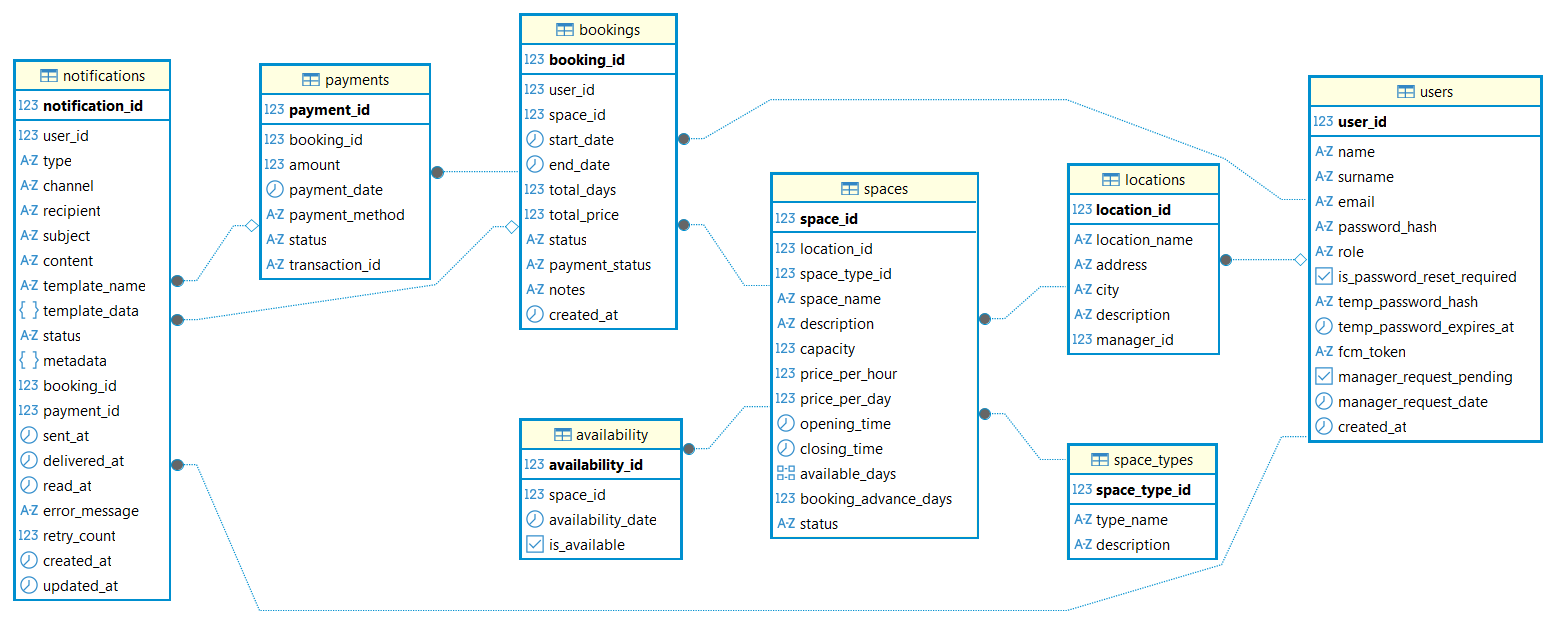
\includegraphics[width=\textwidth]{sections/ER_schema.png}
\caption{Diagramma ER del Sistema CoWorkSpace}
\label{fig:er_diagram}
\end{figure}

\subsection{Relazioni Principali}
\begin{itemize}
    \item \textbf{Users → Locations}: Un manager può gestire più sedi (1:N)
    \item \textbf{Locations → Spaces}: Una sede contiene più spazi (1:N)
    \item \textbf{Space Types → Spaces}: Un tipo può essere utilizzato da più spazi (1:N)
    \item \textbf{Spaces → Availability}: Ogni spazio ha disponibilità per più giorni (1:N)
    \item \textbf{Users → Bookings}: Un utente può fare più prenotazioni (1:N)
    \item \textbf{Spaces → Bookings}: Uno spazio può essere prenotato più volte (1:N)
    \item \textbf{Bookings → Payments}: Ogni prenotazione ha un unico pagamento (1:1)
    \item \textbf{Users → Notifications}: Un utente riceve più notifiche (1:N)
\end{itemize}

\subsection{Implementazione nel Progetto}

\subsubsection{Modelli JavaScript Implementati}
Il sistema CoWorkSpace implementa i seguenti modelli per gestire le operazioni database:

\begin{table}[H]
\centering
\begin{tabular}{@{}ll@{}}
\toprule
\textbf{Modello} & \textbf{File di Implementazione} \\
\midrule
User & \texttt{src/backend/models/User.js} \\
Location & \texttt{src/backend/models/Location.js} \\
Space & \texttt{src/backend/models/Space.js} \\
SpaceType & \texttt{src/backend/models/SpaceType.js} \\
Booking & \texttt{src/backend/models/Booking.js} \\
Payment & \texttt{src/backend/models/Payment.js} \\
Notification & \texttt{src/backend/models/Notification.js} \\
Availability & \texttt{src/backend/models/Availability.js} \\
\bottomrule
\end{tabular}
\caption{Modelli JavaScript del Sistema}
\end{table}

\subsubsection{Servizi di Business Logic}
Il sistema utilizza i seguenti servizi per implementare la logica di business:

\begin{table}[H]
\centering
\begin{tabular}{@{}lp{8cm}@{}}
\toprule
\textbf{Servizio} & \textbf{Responsabilità} \\
\midrule
AuthService & Autenticazione, autorizzazione, gestione ruoli \\
BookingService & Creazione prenotazioni, controllo disponibilità, calcolo prezzi \\
SpaceService & Gestione spazi, ricerca con filtri, validazioni \\
LocationService & Gestione sedi, assegnazione manager \\
NotificationService & Invio notifiche email e push \\
PaymentService & Gestione pagamenti, integrazione gateway \\
\bottomrule
\end{tabular}
\caption{Servizi di Business Logic}
\end{table}

\subsubsection{Validazioni e Constraints Implementati}
Il sistema implementa le seguenti validazioni a livello database e applicazione:

\begin{lstlisting}[caption=Constraint Database Implementati]
-- Validazioni email formato
CHECK (email ~* '^[A-Za-z0-9._%+-]+@[A-Za-z0-9.-]+\.[A-Za-z]{2,}$')

-- Validazioni date prenotazioni
CONSTRAINT booking_date_order CHECK (start_date <= end_date)
CONSTRAINT booking_future_date CHECK (start_date >= CURRENT_DATE)

-- Validazioni stati
CHECK (status IN ('active', 'maintenance', 'inactive'))
CHECK (type IN ('email', 'push', 'sms'))
\end{lstlisting}

\subsubsection{Sistema di Autorizzazioni}
Il sistema implementa un sistema di autorizzazioni a 3 livelli:

\begin{table}[H]
\centering
\begin{tabular}{@{}lp{10cm}@{}}
\toprule
\textbf{Ruolo} & \textbf{Permessi} \\
\midrule
\textbf{User} & Visualizzare spazi, creare prenotazioni, gestire proprio profilo \\
\textbf{Manager} & Tutti i permessi User + gestire location assegnate, spazi delle proprie location, visualizzare prenotazioni delle proprie location \\
\textbf{Admin} & Tutti i permessi + gestire utenti, promuovere manager, accesso completo al sistema \\
\bottomrule
\end{tabular}
\caption{Matrice dei Permessi per Ruolo}
\end{table}

\subsubsection{Configurazione Database}
Il sistema utilizza PostgreSQL con le seguenti configurazioni:

\begin{itemize}
    \item \textbf{Pool di connessioni}: Gestito tramite \texttt{pg} con retry automatico
    \item \textbf{Transazioni}: Supporto completo per operazioni atomiche
    \item \textbf{Prepared statements}: Utilizzo di query parametrizzate per sicurezza
    \item \textbf{Error handling}: Gestione specifica degli errori PostgreSQL
    \item \textbf{Logging}: Monitoraggio query lente e statistiche pool
\end{itemize}